%%%%%%%%%%%%%%%%%%%%%%%%%%%%%%%%%%%%%%%%%%%%%%%%%%%%%%
% A Beamer template for University of Wollongong     %
% Based on THU beamer theme                          %
% Author: Qiuyu Lu                                   %
% Date: July 2024                                    %
% LPPL Licensed.                                     %
%%%%%%%%%%%%%%%%%%%%%%%%%%%%%%%%%%%%%%%%%%%%%%%%%%%%%%
% Customized for Sharif University of Technology     %
%%%%%%%%%%%%%%%%%%%%%%%%%%%%%%%%%%%%%%%%%%%%%%%%%%%%%%


\documentclass[aspectratio=169]{beamer}
\usefonttheme{serif}
%\documentclass[serif]{beamer}  % for 4:3 ratio
\usepackage[T1]{fontenc} 
\usepackage{fourier} % see "http://faq.ktug.org/wiki/uploads/MathFonts.pdf" for other options
\usepackage{hyperref}
\usepackage{latexsym,amsmath,xcolor,multicol,booktabs,calligra}
\usepackage{graphicx,pstricks,listings,stackengine}
\usepackage{lipsum}
\usepackage{tikz}
\usepackage{amsmath}
\usepackage{amssymb}
\usepackage{graphicx}

\author{Ali Sharifi-Zarchi}
\title{Machine Learning (CE 477)}
\subtitle{Fall 2024}
\institute{
    CE Department \\
    Sharif University of Technology
}
%\date{\small \today}
% \usepackage{UoWstyle}
\usepackage{SUTstyle}

% defs
\def\cmd#1{\texttt{\color{red}\footnotesize $\backslash$#1}}
\def\env#1{\texttt{\color{blue}\footnotesize #1}}
\definecolor{deepblue}{rgb}{0,0,0.5}
\definecolor{deepred}{RGB}{153,0,0}
\definecolor{deepgreen}{rgb}{0,0.5,0}
\definecolor{halfgray}{gray}{0.55}

\lstset{
    basicstyle=\ttfamily\small,
    keywordstyle=\bfseries\color{deepblue},
    emphstyle=\ttfamily\color{deepred},    % Custom highlighting style
    stringstyle=\color{deepgreen},
    numbers=left,
    numberstyle=\small\color{halfgray},
    rulesepcolor=\color{red!20!green!20!blue!20},
    frame=shadowbox,
}


\begin{document}

\begin{frame}
    \titlepage
    \vspace*{-0.6cm}
    \begin{figure}[htpb]
        \begin{center}
            
\includegraphics[keepaspectratio, scale=0.25]{pic/sharif-main-logo.png}
        \end{center}
    \end{figure}
\end{frame}
\begin{frame}    
\tableofcontents[sectionstyle=show,
subsectionstyle=show/shaded/hide,
subsubsectionstyle=show/shaded/hide]
\end{frame}

\section{Introduction}

\begin{frame}{Recap: Self-Attention Mechanism}
    \begin{columns}
        \begin{column}{0.5\textwidth}
            \begin{figure}
                \centering
                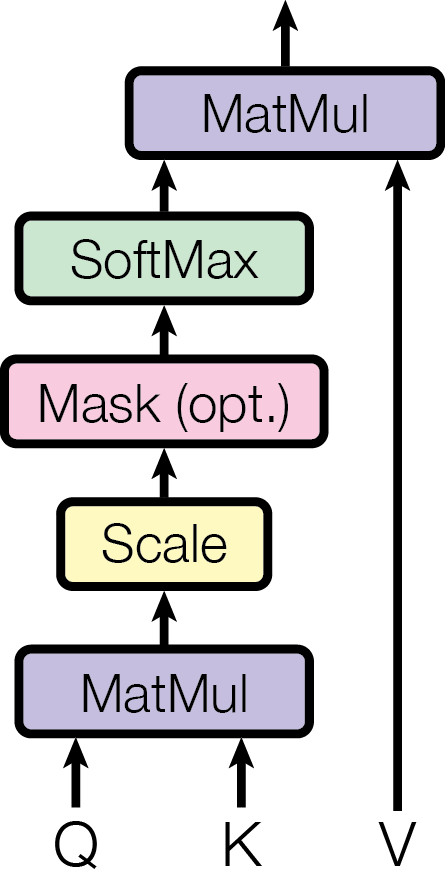
\includegraphics[height=0.75\textwidth]{pic/ModalNet-19}
                \caption{
                Scaled Dot-Product Attention.
                }
                \label{fig:doprod}
            \end{figure}
        \end{column}
        \begin{column}{0.5\textwidth}
            \begin{figure}
                \centering
                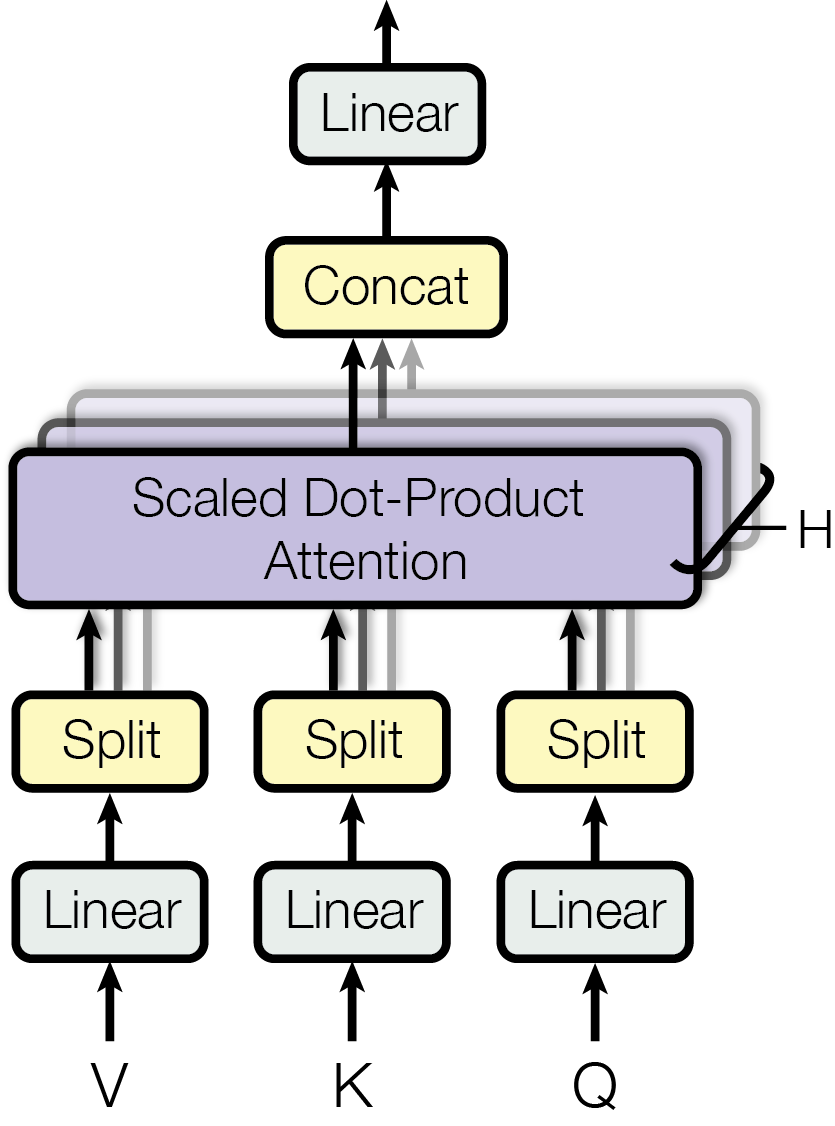
\includegraphics[height=0.75\textwidth]{pic/ModalNet-32}
                \caption{
                Multi-Head Attention consists of several attention layers running in parallel.
                }
                \label{fig:multihead}
            \end{figure}
        \end{column}
    \end{columns}
\end{frame}

% \begin{frame}{Recap: Transformer Architecture}
%     \begin{columns}
%         \begin{column}{0.5\textwidth}
%             \begin{itemize}
%                 \item Transformers have become the model of choice in NLP.
%                 \item The dominant approach is to pre-train on a large text corpus and then fine-tune on a smaller task-specific dataset.
%                 \item Transformers have revolutionized NLP.
%             \end{itemize}
%         \end{column}
%         \begin{column}{0.5\textwidth}
%             \begin{figure}
%                 \centering
%                 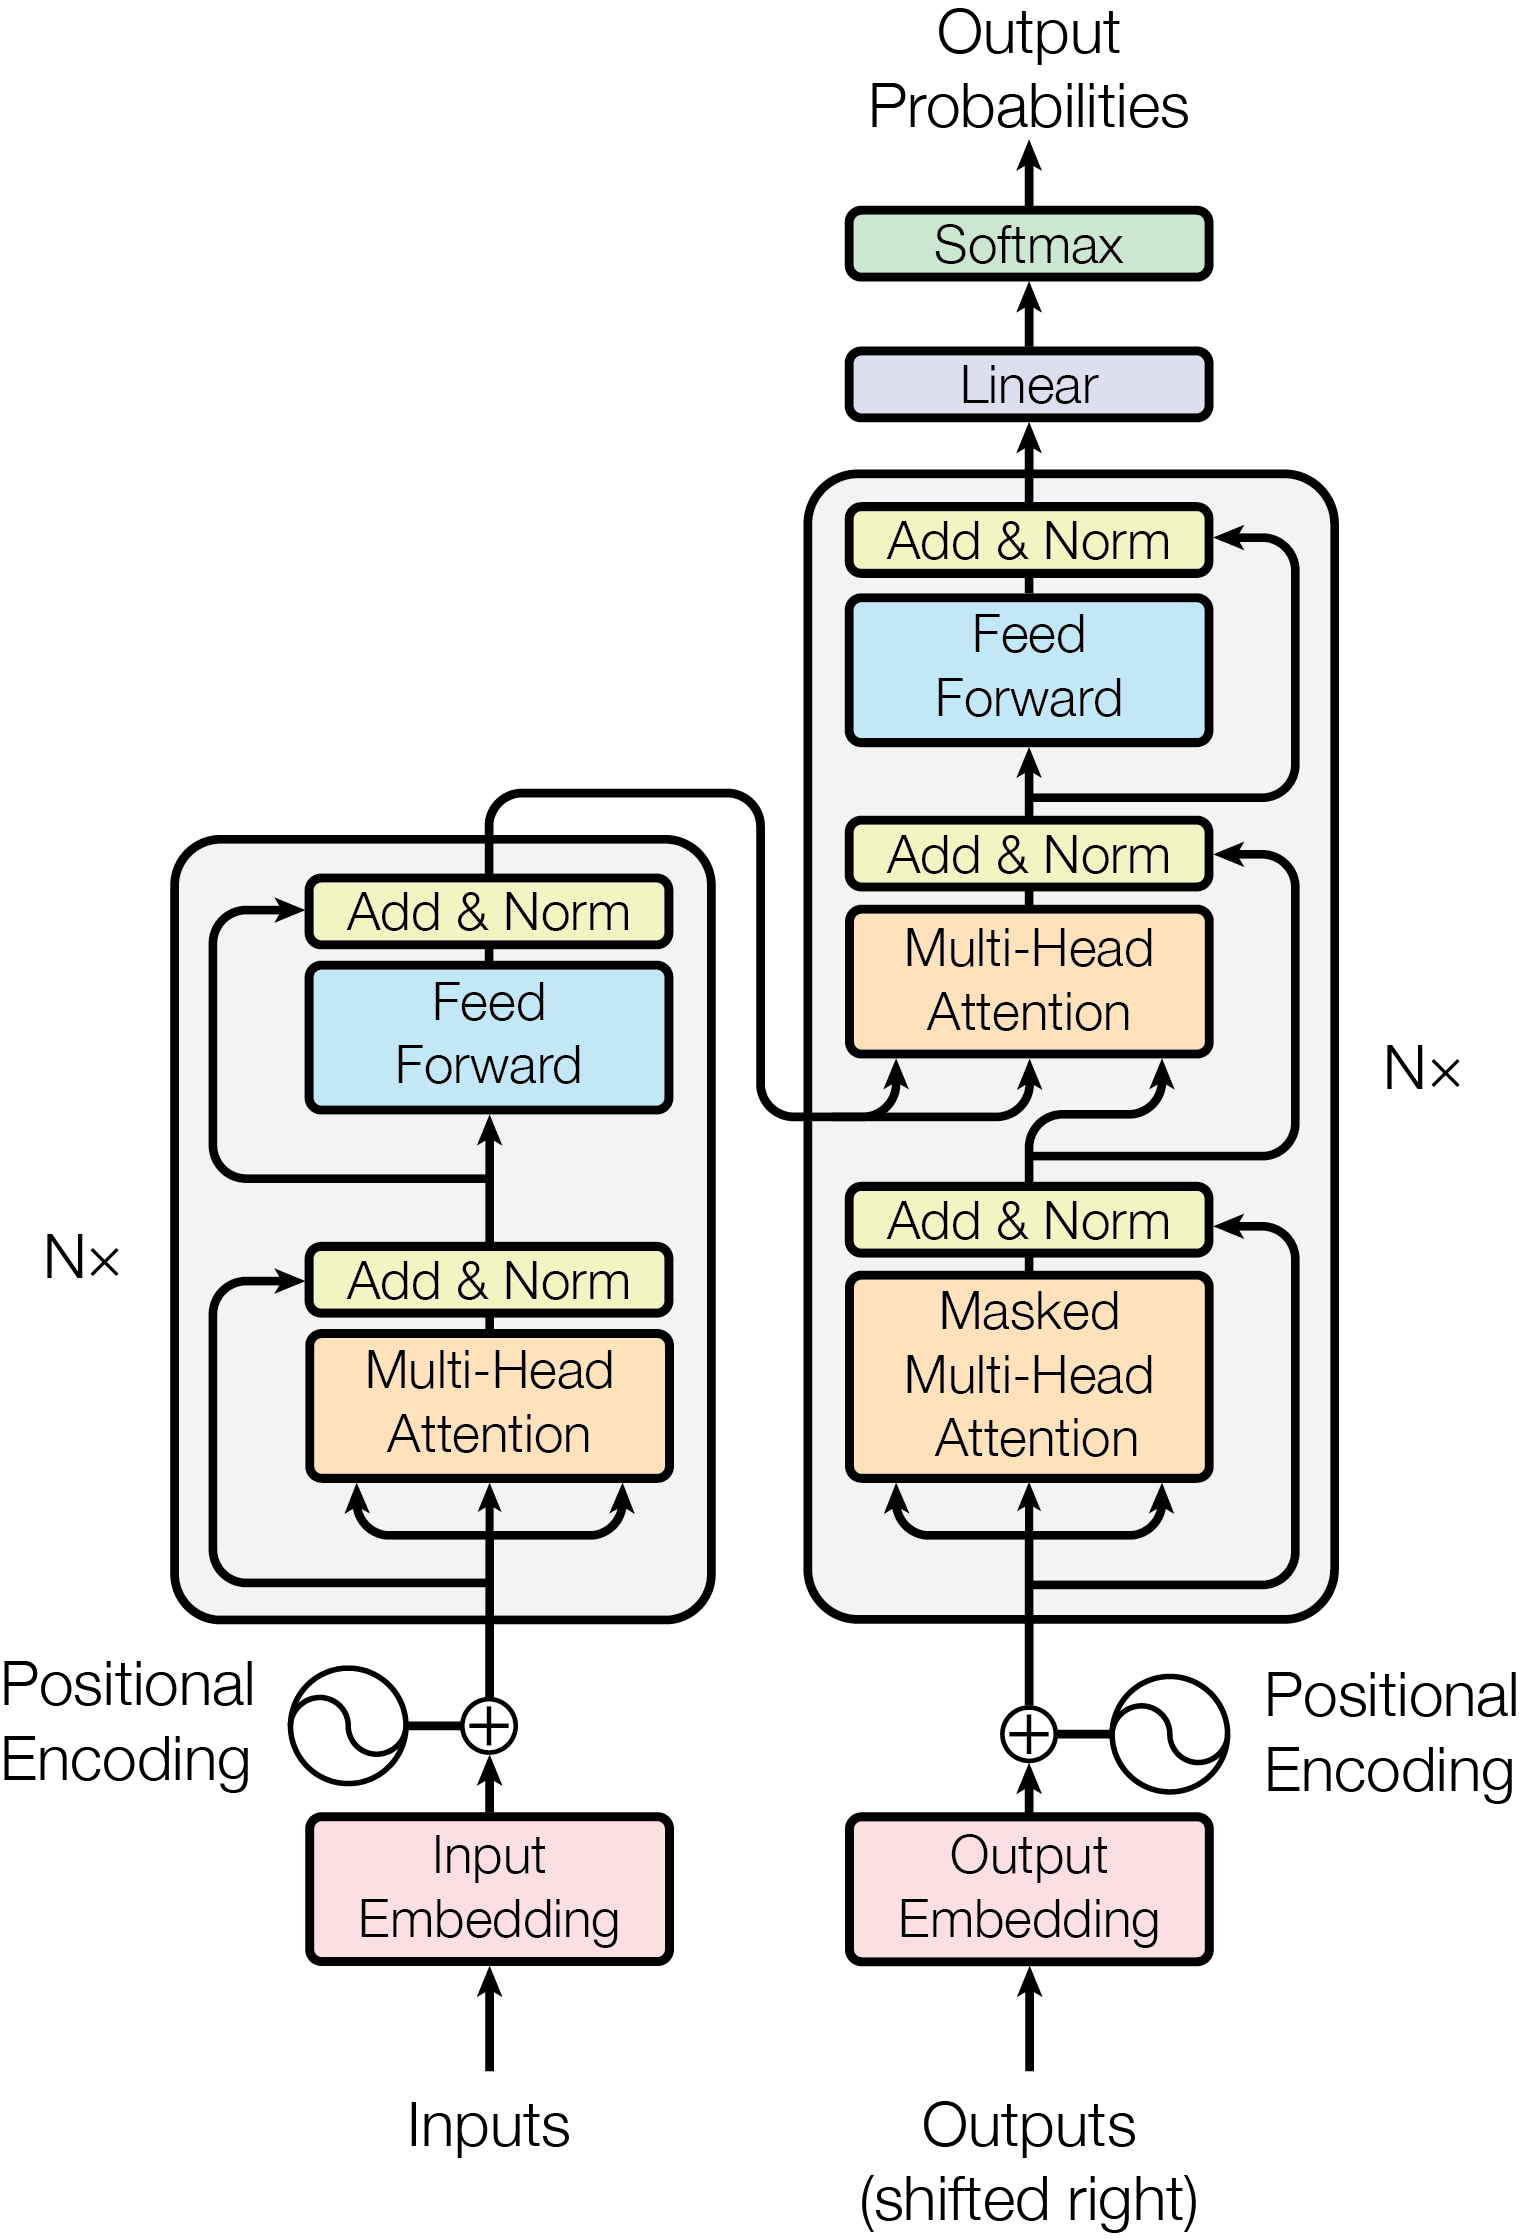
\includegraphics[height=\textwidth]{pic/ModalNet-21}
%                 \label{fig:transformer}
%             \end{figure}
%         \end{column}
%     \end{columns}
% \end{frame}


\begin{frame}{Strengths and Limitations of CNNs}
    \begin{columns}
        \begin{column}{0.55\linewidth}
            \begin{itemize}
                \item CNNs excel at:
                \begin{itemize}
                    \item \emph{Local Feature Extraction} 
                    \item \emph{Translation Invariance} 
                    \item \emph{Efficient Computation} 
                \end{itemize}
                \item However, they have limitations due to:
                \begin{itemize}
                    \item \emph{Limited Receptive Field} 
                    \item \emph{Pooling Information Loss} 
                    \item \emph{Struggle with Global Context} 
                \end{itemize}
            \end{itemize}
        \end{column}
        \begin{column}{0.45\linewidth}
            \begin{figure}
                \centering
                \includesvg[width=\linewidth]{pic/ResNet_block}
                \caption{Block diagram of ResNet}
                \label{fig:resnet}
            \end{figure}
        \end{column}
    \end{columns}
\end{frame}




% \begin{frame}{CNNs Struggle with Global Context}
%     \begin{itemize}
%         \item Why it matters: For tasks that require understanding the entire image (e.g., image classification, where the relationship between distant parts of the image may be important), CNNs often require deep architectures to get the full picture.
%         \item Feature Hierarchy: CNNs build a hierarchical structure of features but rely on many layers to achieve global understanding, leading to more complexity.
%     \end{itemize}
% \end{frame}



\section{Transformers for Vision}

\begin{frame}{Transformers: From Language to Vision}
    \begin{itemize}
        \item The Transformer architecture was designed for \textbf{sequence-to-sequence learning}.
        \item Transformers have revolutionized NLP and become the model of choice.
        % \item Transformers emerged as the model of choice in various \textbf{NLP} tasks and had a revolutionizing effect.
        % \item In the field of \textbf{Computer Vision} however, the dominant architecture has remained the CNN.
	    \item Is it possible to do adapt the Transformer for image data?
    \end{itemize}
\end{frame}


\begin{frame}{Idea \#1: Add Attention to Existing CNNs}
    \begin{itemize}
        \item Model is still a CNN!
    \end{itemize}
    \begin{figure}
        \centering
        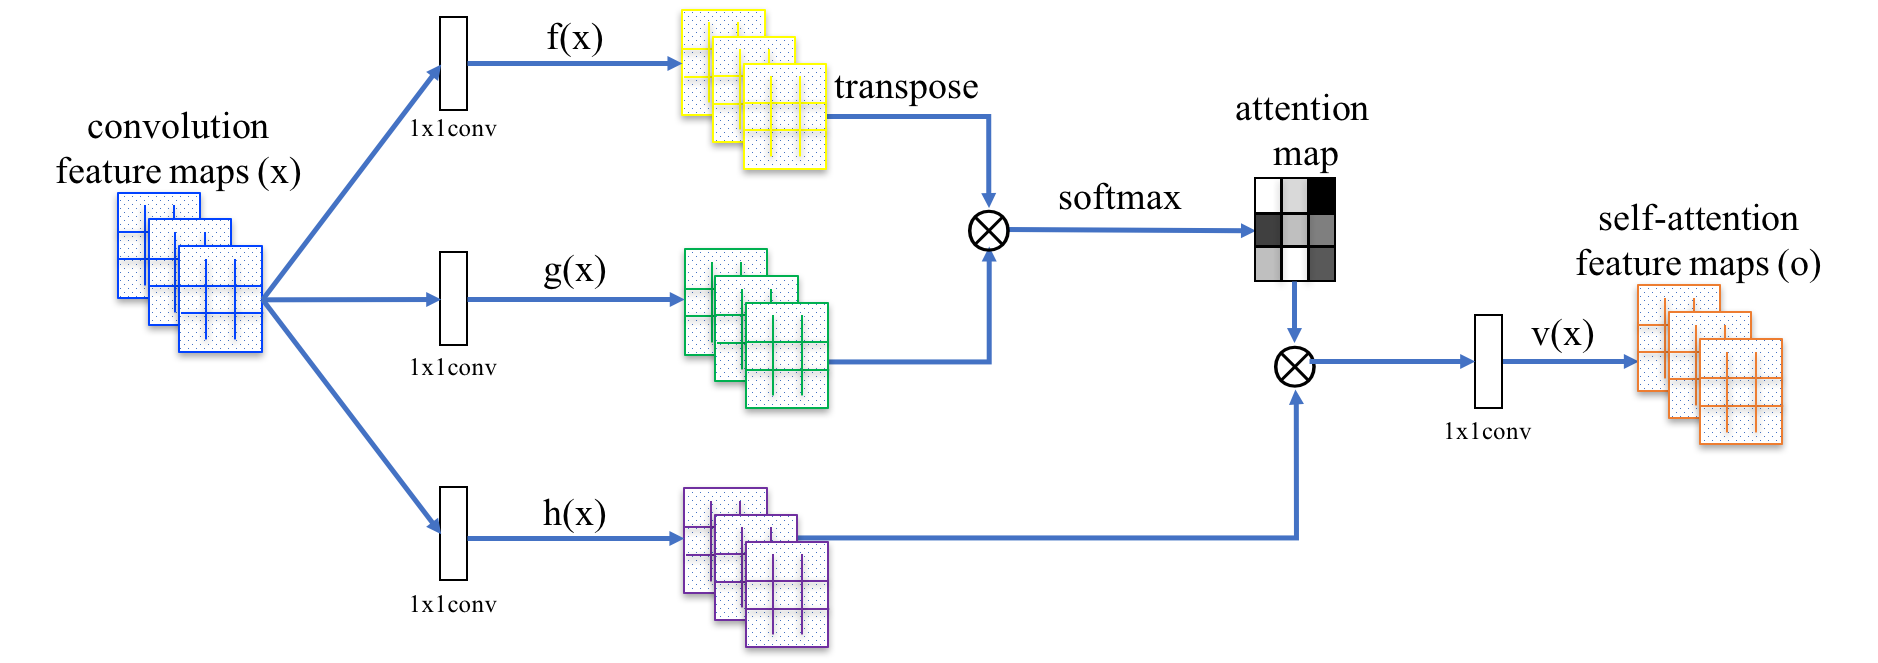
\includegraphics[width=\linewidth]{pic/framework}
        % \caption{Add Self-Attention blocks between existing ResNet blocks.}
        \label{fig:idea1}
    \end{figure}
\end{frame}

\begin{frame}{Idea \#2: Replace Convolution with “Local Attention”}
    \begin{itemize}
        \item Lots of tricky details, hard to implement, only marginally better than ResNets.
    \end{itemize}
    \begin{figure}
        \centering
        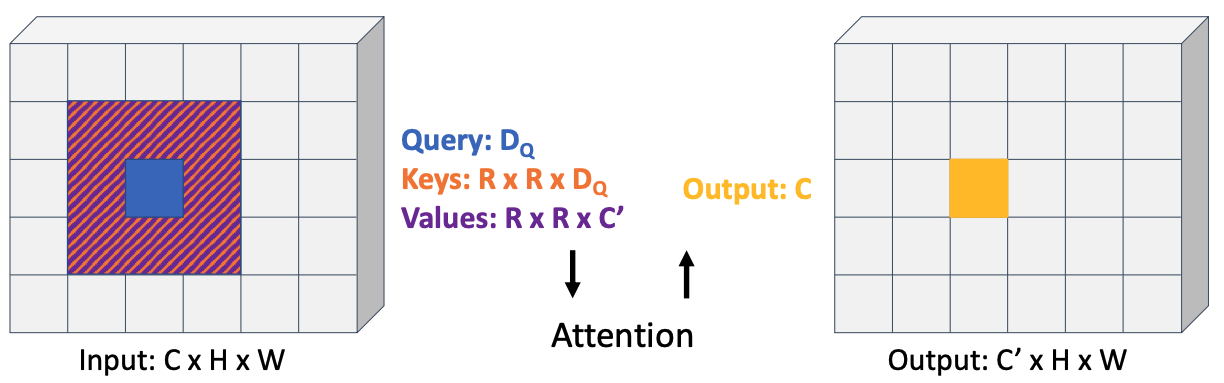
\includegraphics[width=\linewidth]{pic/idea2}
        % \caption{Replace all convolutional layers in CNNs with local attention.}
        \label{fig:idea1}
    \end{figure}
\end{frame}


\begin{frame}{Idea \#3: Standard Transformers on Pixels}
    \begin{itemize}
        \item Insane memory usage!
    \end{itemize}
    \begin{figure}
        \centering
        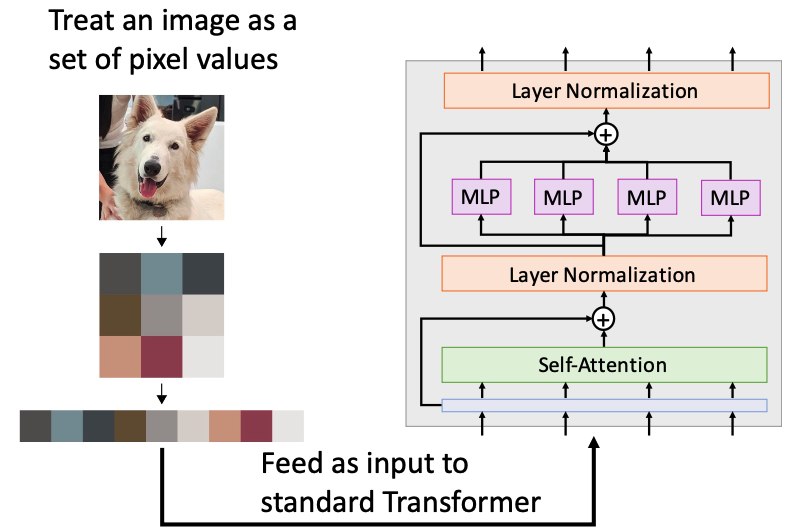
\includegraphics[width=0.5\linewidth]{pic/idea3}
        % \caption{Treat each image pixel as an input token for the transformer.}
        \label{fig:idea1}
    \end{figure}
\end{frame}


\begin{frame}{Idea \#4: Standard Transformer on Patches}
    \begin{itemize}
        % \item Follow the original Transformer as closely as possible.
        \item Fixes idea \#1 by entirely replacing convolutional layers.
        \item Fixes idea \#2 by simplifying implementation.
        \item Fixes idea \#3 by reducing memory usage.
        \item This is the main idea behind \textbf{Vision Transformers}!
    \end{itemize}
\end{frame}

\section{How ViT Works?}

\begin{frame}{Processing Text}
    \begin{itemize}
        \item \textbf{Token Embeddings}: The input text is broken down into individual tokens (e.g., words, sub-words). Each token is analogous to a patch in an image.
	    \item \textbf{Word Embeddings}: Each token is converted into a fixed-length vector representation (embedding) using a technique like Word2Vec, GloVe, or learned embeddings within the transformer model itself.
	    \item \textbf{Self-Attention on Tokens}: The transformer's self-attention mechanism is applied to these word embeddings. This allows the model to capture relationships between different words in the sentence, understanding context and dependencies.
    \end{itemize}
\end{frame}

\begin{frame}{Processing Images}
    \begin{itemize}
        \item \textbf{Patch Embeddings}: ViT splits an image into fixed-size patches (e.g., 16x16 pixels). Each patch is treated like a token in NLP, much like words in a sentence.
	    \item \textbf{Linear Embedding}: Each patch is flattened into a 1D vector and then linearly projected to a fixed-length embedding.
	    \item \textbf{Self-Attention on Patches}: The Transformer’s self-attention mechanism is then applied to these patch embeddings, allowing the model to learn relationships between patches.
    \end{itemize}
\end{frame}

\begin{frame}{ViT Overview}
    \begin{figure}
        \centering
        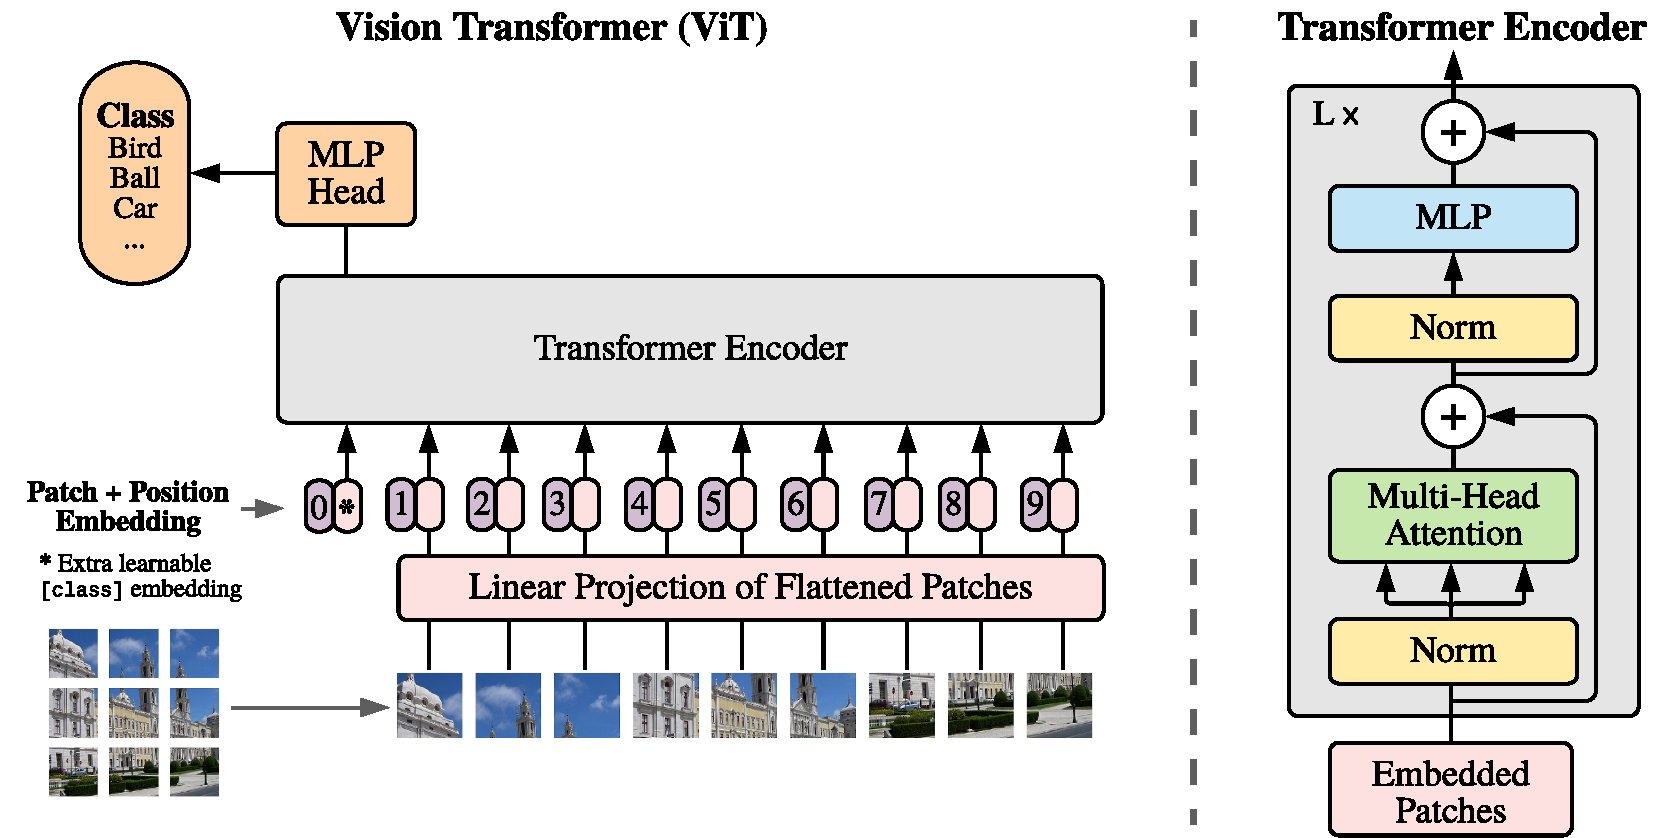
\includegraphics[width=0.95\linewidth]{pic/model_scheme}
        % \caption{We split an image into fixed-size patches, linearly embed each of them, add position embeddings, and feed the resulting sequence of vectors to a standard Transformer encoder. In order to perform classification, we use the standard approach of adding an extra learnable “classification token” to the sequence.}
        \label{fig:vit-figure}
    \end{figure}
\end{frame}

\begin{frame}{Positional Encoding}
    \begin{itemize}
        \item Positional Encoding: Since Transformers process all patches simultaneously (losing the inherent spatial structure of the image), positional encodings are added to the patch embeddings to maintain the relative position of each patch.
	    \item Global Awareness with Position Information: These encodings allow the Transformer to understand not just the content of the patches, but where each patch is located within the image.
    \end{itemize}
\end{frame}

\begin{frame}{Inspecting Vision Transformer}
    \begin{columns}
        \begin{column}{0.5\textwidth}
            \begin{itemize}
                \item Self-attention allows ViT to integrate information across the entire image even in the lowest layers.
            \end{itemize}
        \end{column}
        \begin{column}{0.5\textwidth}
            \begin{figure}
                \centering
                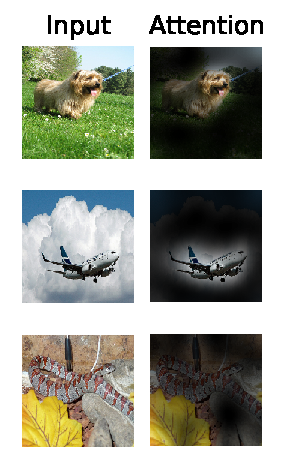
\includegraphics[height=0.75\textwidth]{pic/20201002_selected_attention_examples}
                \caption{Representative examples of attention from the output token to the input space.}
                \label{fig:inspecting-vit}
            \end{figure}
        \end{column}
    \end{columns}
\end{frame}

\begin{frame}{Inductive Bias}
    \begin{itemize}
        \item In CNNs, locality, two-dimensional neighborhood structure, and translation equivariance are baked into each layer throughout the whole model.
        \item In ViT, only MLP layers are local and translationally equivariant, while the self-attention layers are global.
        \item The two-dimensional neighborhood structure is used very sparingly
    \end{itemize}
\end{frame}

\input{sections/4_Image_Captioning}

\section{Vision Transformer vs. CNN}

\begin{frame}{ViT vs. CNN}
    \begin{itemize}
        \item Local vs. Global Understanding: While CNNs are good at local feature extraction, ViT captures global relationships from the very first layer.
	    \item Efficiency on Large Datasets: ViT shines on large datasets, while CNNs, due to their inductive biases (local patterns, translation invariance), perform better on smaller datasets without needing as much data.
	    \item Simplicity in Architecture: ViT uses a simpler architecture with fewer specialized layers, while CNNs rely on task-specific layers like convolutions and pooling.
    \end{itemize}
\end{frame}

\begin{frame}{Combining CNNs and Transformers}
    \begin{itemize}
        \item As an alternative to raw image patches, the input sequence can be formed from feature maps of a CNN.
	    \item These hybrid models combine the local feature extraction capabilities of CNNs with the global context awareness of Transformers. 
        \item These models can perform well even on smaller datasets.
    \end{itemize}
\end{frame}

\begin{frame}{Dataset Size}
    \begin{columns}
        \begin{column}{0.5\textwidth}
            \begin{figure}
                \centering
                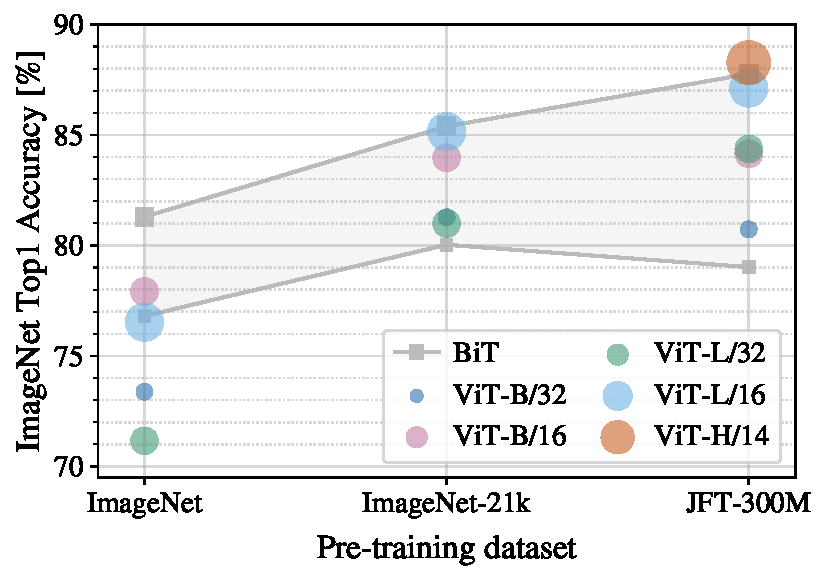
\includegraphics[width=\textwidth]{pic/transvolution-i1k-scaling}
                \caption{
                % Transfer to ImageNet. 
                While large ViT models perform worse than BiT ResNets when pre-trained on small datasets, they shine when pre-trained on larger datasets. 
                %Similarly, larger ViT variants overtake smaller ones as the dataset grows.
                }
                \label{fig:transvolution}
            \end{figure}
        \end{column}
        \begin{column}{0.5\textwidth}
            \begin{figure}
                \centering
                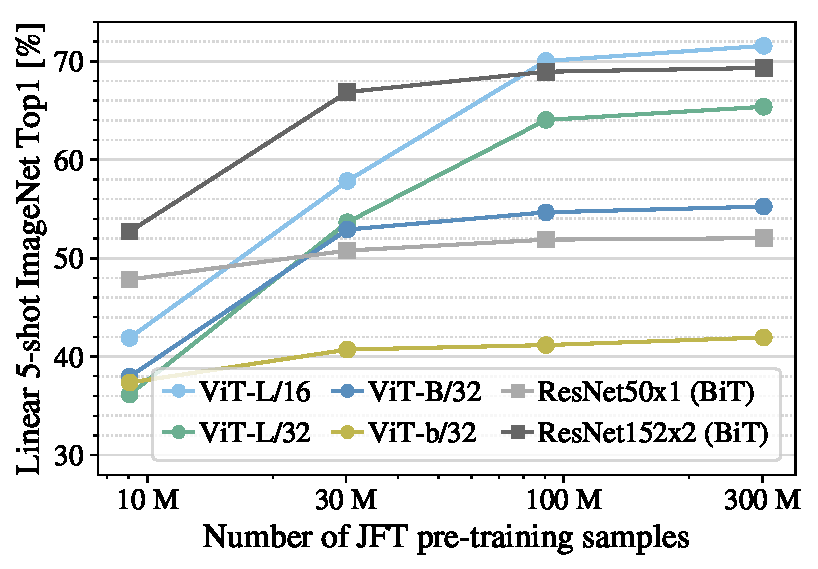
\includegraphics[width=\textwidth]{pic/imagenet_5shot}
                \caption{
                % Linear few-shot evaluation on ImageNet versus pre-training size. 
                ResNets perform better with smaller pre-training datasets but plateau sooner than ViT, which performs better with larger pre-training. 
                %ViT-b is ViT-B with all hidden dimensions halved.
                }
                \label{fig:imagenet_5shot}
            \end{figure}
        \end{column}
    \end{columns}
\end{frame}


\begin{frame}{Performance versus Pre-training}
    \begin{figure}
        \centering
        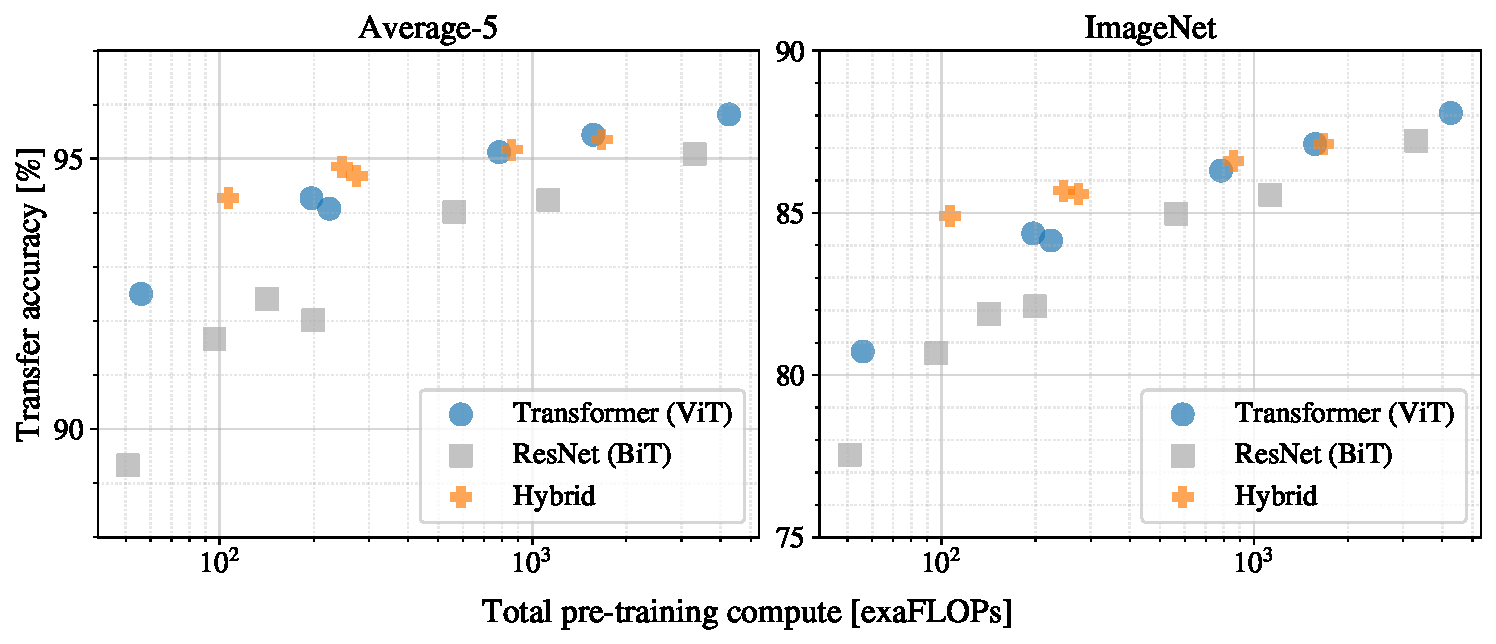
\includegraphics[width=0.9\linewidth]{pic/finetune_vs_compute2.pdf}
        \caption{Vision Transformers generally outperform ResNets with the same computational budget. Hybrids improve upon pure Transformers for smaller model sizes, but the gap vanishes for larger models.}
        \label{fig:enter-label}
    \end{figure}
\end{frame}

\section{References}

\begin{frame}{Contributions}
    \begin{itemize}
        \item These slides have been prepared thanks to: 
	    \begin{itemize}
	        \item Ramtin Moslemi
            \item Ashkan Majidi
	    \end{itemize}
    \end{itemize}
\end{frame}


\begin{frame}{References}
    \bibliography{ref}
    \bibliographystyle{ieeetr}
    \nocite{*}
\end{frame}

\end{document}